
\section{11. Diagrama de Gantt}
\label{sec:gantt}

Debido a que todas las tareas serán realizadas por el responsable del proyecto (es decir, una sola persona) las dependencias de las actividades del diagrama de \textit{Activity on Node} fueron adaptadas para reflejar la imposibilidad de ejecutar tareas en paralelo.

El diagrama de Gantt se muestra separado en dos partes. Un cuadro \ref{tab:wbs} que contiene el desglose de tareas y la figura \ref{fig:Gantt} que contiene el diagrama propiamente dicho.

\begin{table}[ht]
  \centering

  \begin{tabularx}{\linewidth}{@{}|c|X|c|c|@{}}
    \hline
    \rowcolor[HTML]{C0C0C0}
    WBS & \multicolumn{1}{c|}{\cellcolor[HTML]{C0C0C0}Nombre} & Inicio  & Fin     \\ \hline
    1.1 & Definición de requerimientos con el cliente & 01/08/23 & 01/08/23 \\ \hline
    1.2 & Planificación & 03/08/23 & 12/08/23 \\ \hline
    2.1 & Recopilación de documentación online & 13/08/23 & 14/08/23\\ \hline
    2.2 & Lectura y comprensión de los documentos & 15/08/23 & 19/08/23\\ \hline
    2.3 & Capacitación sobre el conjunto de instrucciones del procesador & 20/08/23 & 29/08/23\\ \hline
    3.1 & Creación del repositorio de desarrollo & 30/08/23 & 30/08/23\\ \hline
    3.2 & Creación del ambiente de CI/CD para tests & 31/08/23 & 01/09/23\\ \hline
    3.3 & Desarrollo  del ambiente CI/CD para documentación & 02/09/23 & 04/09/23\\ \hline
    3.4 & Creación del ambiente de CI/CD para empaquetado & 05/09/23 & 06/09/23\\ \hline
    4.1 & Revisión y análisis de código existente & 07/09/23 & 12/09/23\\ \hline
    4.2 & Selección del código a reutilizar e importación & 13/09/23 & 25/09/23\\ \hline
    4.3 & Refactorización del código & 27/09/23 & 28/09/23\\ \hline
    5.1 & Lectura de documentación & 29/09/23 & 08/10/23\\ \hline
    5.2 & Internalización con su API & 09/10/23 & 18/10/23\\ \hline
    5.3 & Pruebas de límites y alcances del framework & 19/10/23 & 23/10/23\\ \hline
    6.1 & Desarrollo de modelos de periféricos & 24/10/23 & 11/11/23\\ \hline
    6.2 & Desarrollo de modelos de memorias y registros & 12/11/23 & 25/11/23\\ \hline
    6.3 & Desarrollo de instrucciones & 26/11/23 & 16/01/24\\ \hline
    7.1 & Pruebas unitarias de modelos & 17/01/24 & 26/01/24\\ \hline
    7.2 & Pruebas unitarias de instrucciones & 27/01/24 & 14/02/24\\ \hline
    7.3 & Pruebas de API & 15/02/24 & 24/02/24\\ \hline
    7.4 & Corrección de errores & 25/02/24 & 29/02/24\\ \hline
    8.1 & Creación del manual de usuario & 01/03/24 & 19/03/24\\ \hline
    8.2 & Documentación de API en Doxygen & 20/03/24 & 24/03/24\\ \hline
    9.1 & Preparación de las memorias & 25/03/24 & 12/04/24\\ \hline
    9.2 & Redacción de las memorias & 13/04/24 & 01/05/24\\ \hline
    9.3 & Presentación del trabajo & 02/05/24 & 16/05/24\\ \hline
  \end{tabularx}
  \caption{Desglose de tareas.}
  \label{tab:wbs}
\end{table}


\begin{landscape}

  \begin{figure}[htpb]
    \centering
    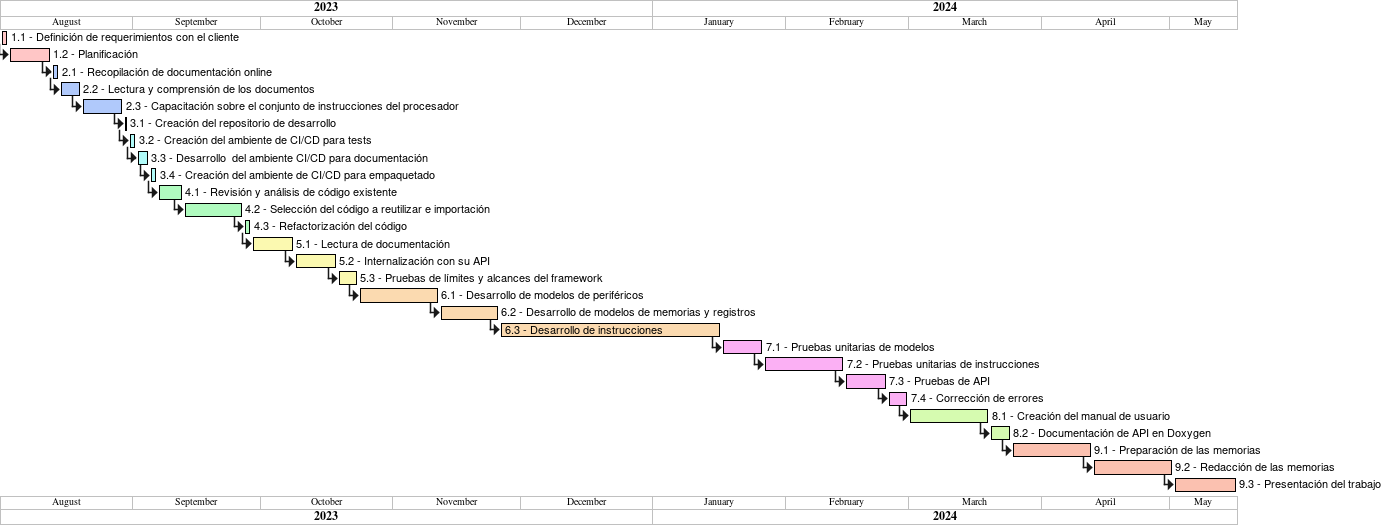
\includegraphics[width=1.5\textwidth]{./assets/Gantt.png}
    \caption{Diagrama de Gantt.}
    \label{fig:Gantt}
  \end{figure}

  \vspace{25px}


\end{landscape}
